% truth table -> K-map -> minimal expression pipeline
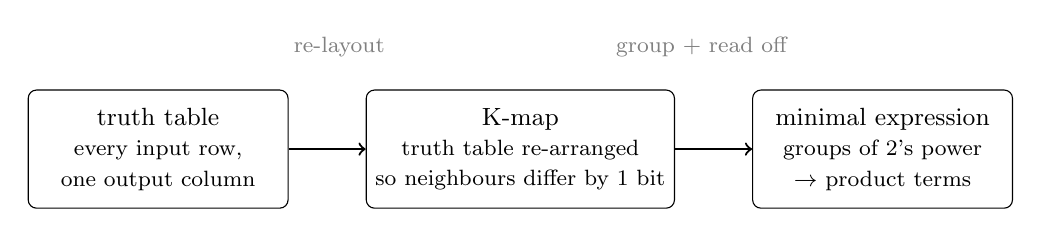
\begin{tikzpicture}[font=\small, box/.style={draw, rounded corners=3pt, align=center, minimum height=1.5cm, minimum width=3.3cm}]
\node[box] (tt) at (0,0) {truth table\\ \footnotesize every input row,\\ \footnotesize one output column};
\node[box] (km) at (4.6,0) {K-map\\ \footnotesize truth table re-arranged\\ \footnotesize so neighbours differ by 1 bit};
\node[box] (ex) at (9.2,0) {minimal expression\\ \footnotesize groups of 2's power\\ \footnotesize $\to$ product terms};
\draw[->, thick] (tt) -- (km);
\draw[->, thick] (km) -- (ex);
\node[font=\footnotesize, text=gray] at (2.3,1.3) {re-layout};
\node[font=\footnotesize, text=gray] at (6.9,1.3) {group + read off};
\end{tikzpicture}
